\chapter{Energieflexibilisierung, Strommarktdesign und wässrige Teilreinigung: Grundlagen}
\label{ch_03Energieflexibilisierung, Strommarktdesign und wässrige Teilreinigung: Grundlagen}

In diesem Kapitel werden die für diese Masterarbeit notwendigen theoretischen Grundlagen und Definitionen beschrieben. Diese bilden die Basis für die in Kapitel \ref{ch_06Techno-ökonomische Analyse} durchgeführte techno-ökonomische Analyse sowie für die Konzeptentwicklung. In Kapitel \ref{ch_03Demand-Response und Energieflexibilisierung} erfolgt die Definition der Konzepte Demand-Response und der Energieflexibiliserung. Zudem werden die Funktionen der Anpassung von Verbrauchslasten und die Glättung von Lastspitzen detailliert beschrieben. Im Fokus stehen in Kapitel \ref{ch_03Strommarktdesign und Wetterprognosen} das grundlegende Strommarktdesign und der Einfluss von Wetterprognosen auf die Effektivität der Energieflexibilisierung. Kapitel \ref{ch_03Wässrige Teilreinigung} befasst sich mit der wässrigen Teilreinigung und erläutert die Anwendung von Energieflexibilisierung sowohl an Durchlaufreinigungsanlagen (DLRA) als auch an Ein-Bad-Reinigungsmaschinen. Um ein besseres Verständnis für die Umsetzung der Energieflexibilisierungsmaßnahmen auf der MES-Ebene zu bekommen, ist in Kapitel \ref{ch_03Industrielle Kommunikation über die OPC UA Schnittstelle} eine Einführung in die industrielle Kommunikation über die OPC UA Schnittstelle notwendig.


\section{Demand-Response und Energieflexibilisierung}
\label{ch_03Demand-Response und Energieflexibilisierung}

In der Literatur werden die Begriffe Demand-Response und Energieflexibilsierung häufig im gleichen Kontext verwendet. Es folgen die Definitionen beider Begriffe und eine differenzierte Ansicht darauf, wie und ob sie sich unterscheiden.\\

Energieflexibilität ist definiert als: \glqq Fähigkeit eines Produktionssystems sich schnell und prozesseffizient an Änderungen des Energiemarktes anzupassen.\grqq~\cite{VDI5207Blatt2020}
Die Produktqualität wird durch diese Eignung nicht signifikant beeinflusst.\\


Im Kontext der Energieflexibilisierung ist es maßgeblich die Begriffe Energieflexibilitätsmaßnahme und Energieflexibilitätspotenzial voneinander abzugrenzen. Eine bestimmte Anlage oder eine gesamte Fabrik kann entsprechend in dem Maße der Höhe des jeweiligen Energieflexibilitätspotenzials energieflexibel betrieben werden. Das bedeutet, dass die Fähigkeit zur Anpassung an variable Energiebedingungen direkt vom vorhandenen Energieflexibilitätspotenzial abhängt. Es beschreibt den Umfang der veränderbaren Last unter vorherrschenden Rahmenbedingungen \cite{VDI5207Blatt2020}. Für eine präzise Beurteilung des Energieflexibilitätspotenzials ist eine Abgrenzung des Potenzials wie in Abbildung \ref{fig_03Potenzialbegriffe} von hoher Relevanz.\\

\begin{figure}[h]
	\centering
	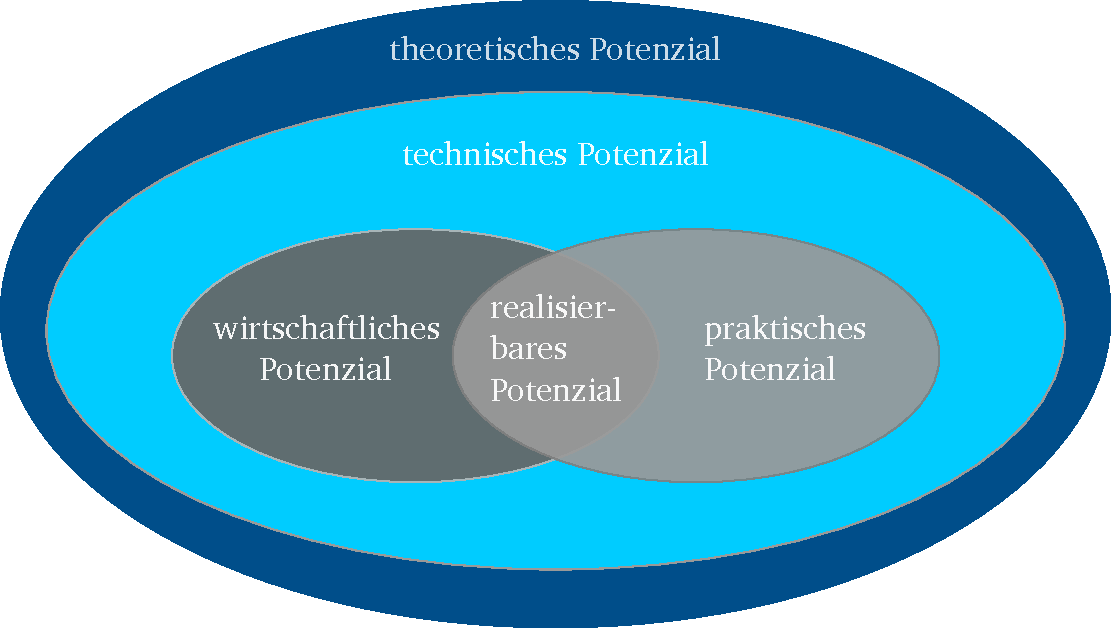
\includegraphics[width=400pt]{figures/03_Grundlagen/Potenzialbegriffe.pdf}
	\caption{Potenzialbegriffe, nach \cite{VDI5207Blatt2020}}
	\label{fig_03Potenzialbegriffe}
\end{figure}

Wie in der Abbildung \ref*{fig_03Potenzialbegriffe} dargestellt, umfasst das theoretische Potenzial sämtliche anderen Potenziale. Es handelt sich um eine berechnete Größe, die sich aus der Anschlussleistung aller Endenergieformen ergibt. Unter Endenergie werden die gehandelten und dem Markt entzogenen Energieträger verstanden. Sie dienen primär der Herstellung und Transformation von Nutzenergie. Das technische Potenzial ist ein wenig differenzierter als das theoretische Potenzial. Hier liegt der Fokus auf den Energieanforderungen, welche an die jeweiligen technologischen Rahmenbedingungen angepasst werden. Das heißt, es werden entsprechende Parameter der Anlagen variiert, um somit die Leistungsaufnahme und die einzelnen Zeitintervalle zu steuern \cite{VDI5207Blatt2020}.\\

Auf der tiefsten Ebene sind das wirtschaftliche und praktische Potenzial dargestellt. Beide Potenziale sind Teilmengen des technischen Potenzials. In der wirtschaftlichen Betrachtung wird der Teil des technischen Potenzials untersucht, welcher auch ökonomisch genutzt werden kann. Dieses Potenzial kann nur genutzt werden, wenn der Break-Even-Punkt überschritten wird und somit die Erlöse durch die Nutzung der Energieflexibilität die Kosten übersteigen. Die praktische Ansicht betrachtet ebenfalls eine Teilmenge des technischen Potenzials. Sie berücksichtigt geschäftliche, regulatorische und administrative Einschränkungen. Die Schnittmenge des wirtschaftlichen und des praktischen Potenzials bildet das realisierbare Potenzial ab. Hier wird untersucht, wie Energieflexibilität wirtschaftlich sinnvoll unter den bestehenden Unternehmenseinschränkungen eingesetzt werden kann \cite{VDI5207Blatt2020}.\\

Diese Arbeit beinhaltet eine Energieflexibilitäts- bzw. Demand-Response Analyse, welches das technische Potenzial der betrachteten DLRA untersucht um festzulegen, welche Elemente der Anlage für die Energieflexibilisierung zur Verfügung stehen, siehe Kapitel \ref{ch_06Bewertung verschiedener Flexibilitätsziele und deren technologische Umsetzungsmöglichkeiten}. Um das wirtschaftliche Potenzial zu analysieren, werden in Kapitel \ref{ch_06Wirtschaftliche Analyse der Maßnahmen} verschiedene Energieflexibilitätsmaßnahmen ökonomisch bewertet um dann zu entscheiden, welche auf der MES-Ebene umgesetzt werden sollen \cite{VDI5207Blatt2020}.\\

Um die verschiedenen Energieflexibilitätspotenziale nutzen zu können, werden passende Energieflexibilitätsmaßnahmen ausgewählt und auf den verschiedenen Ebenen der Automatisierungspyramide umgesetzt. Eine Energieflexibilitätsmaßnahme ist eine gezielte Handlung, um einen spezifischen Zustandswechsel in einem Produktionssystem zu bewirken. Dieser Vorgang umfasst den Zustandswechsel einer Produktionsstation sowie die daraus resultierenden Wechselwirkungen innerhalb des Produktionssystems \cite{VDI5207Blatt2020}. Die VDI-Richtlinie der Deutschen Ingenieure e.V. \cite{VDI5207Blatt2020} hat 16 verschiedene Energieflexibilitätsmaßnahmen definiert, welche in der Automatisierungspyramide drei verschiedene Ebenen zugeordnet werden, 

\begin{figure}[H]
	\centering
	\includegraphics[width=\textwidth]{figures/03_Grundlagen/Energieflexibilitätsmaßnahmen in der energieflexiblen Fabrik.pdf}
	\caption{Energieflexibilitätsmaßnahmen in der energieflexiblen Fabrik, nach \cite{VDI5207Blatt2020}}
	\label{fig_03Energieflexibilitätsmaßnahmen in der energieflexiblen Fabrik}
\end{figure}

siehe Abbildung \ref{fig_03Energieflexibilitätsmaßnahmen in der energieflexiblen Fabrik}. Neben der Zuweisung der Maßnahmen auf den Ebenen, zeigt die Abbildung \ref{fig_03Energieflexibilitätsmaßnahmen in der energieflexiblen Fabrik} eine Untergliederung dieser anhand eines zeitlichen Horizonts.\\

Im folgenden werden die in Abbildung \ref{fig_03Energieflexibilitätsmaßnahmen in der energieflexiblen Fabrik} visualisierten Maßnahmen im Detail beschrieben. Die unterste Ebene der Automatisierungspyramide wird als Fertigungsebene bezeichnet. Auf dieser Ebene werden Maßnahmen innerhalb eines kurzfristigen Zeithorizonts von einer Minute bis zu einer Stunde implementiert \cite{VDI5207Blatt2020}. 

\begin{itemize}[label={--}]
	\item \textbf{Prozess unterbrechen}: \\Diese Maßnahme beinhaltet temporäre Unterbrechung des Produktionsprozesses bzw. einzelner Verbraucher. 
	\item \textbf{Prozessparameter anpassen}:\\Die Justierung der Prozessparameter erlaubt die Modifikation des Leistungsbedarfs, ohne dass zusätzlicher Energieeinsatz nachgeholt werden muss.
	\item \textbf{Bearbeitungsreihenfolge ändern}:\\ Die Variation der Bearbeitungsreihenfolge in den Prozessschritten zielt darauf ab, unterschiedliche Leistungsbedarfe innerhalb der Produktionsherstellung zu nutzen.
	\item \textbf{Energie speichern inhärent}:\\Die Verwendung von Toleranzen verschiedener Zustandsgrößen in Prozessen als Energiespeicher ermöglicht die bewusste Speicherung von Energie in einem passenden inhärenten Speichermedium.
	\item \textbf{Energiebivalent betreiben}:\\ Der Einsatz diverser Nutzenergieformen innerhalb der anlagenspezifischen Produktionsprozesse.
\end{itemize}

In den Produktionsprozessen werden Energieflexibilitätsmaßnahmen auf der Fertigungsleitebene durchgeführt, wobei diese Maßnahmen einen Zeithorizont von einigen Stunden bis zu einer Woche haben. In dieser Arbeit soll ein Konzept zur Umsetzung von ausgewählten Flexibilitätsmaßnahmen auf der MES-Ebene entwickelt werden. Deswegen werden die möglichen Maßnahmen auf der Fertigungsleitebene nicht nur definiert, sondern auch die Voraussetzung für die Umsetzung beschrieben. 

\begin{itemize}[label={--}]
	\item \textbf{Auftragsstart verschieben}: \\Das Verschieben des Auftragsstarts bezieht sich auf das frühere oder spätere Beginnen von Aufträgen innerhalb längerer Zeiträume. Dabei werden freie Produktionskapazitäten genutzt, um zusätzliche Aufträge in der jeweiligen Periode zu bearbeiten. 
	
	Für eine erfolgreiche Implementierung sind ausreichend Puffer in der retrospektiven Planung zur Fertigstellung erforderlich. Das bedeutet, die jeweiligen Aufträge befinden sich nicht auf dem zeitkritischen Pfad und es sind genügend Lagerkapazitäten für die Zwischenlagerung vorhanden.
	\item \textbf{Auftrag unterbrechen (min-h-d)}: \\Im Fall der Auftragsunterbrechung werden kürzere Zeiträume berücksichtigt. Für die kurzfristige Unterbrechung der Aufträge werden Zeitreserven im Produktionsablauf verwendet. 
	
	Die Maßnahme sollte nur umgesetzt werden, wenn die Möglichkeit für eine Unterbrechung der Produktionskette überhaupt besteht. Es dürfen keine Schäden an der Anlage oder Qualitätsverluste an den Produkten entstehen. 
	\item \textbf{Ressourcenbelegung anpassen}: \\Bei der Anpassung der Ressourcenbelegung werden Produktionsanlagen auf Grundlage ihres Energiebedarfs gezielt ausgewählt. 
	
	Dafür ist eine optimierte Kommunikation zwischen den Maschinen erforderlich. Dadurch wird vermieden, nachfolgenden Produktionsprozesse zu verzögern und somit Qualitäts- sowie Produktivitätsanforderungen zu verletzen.
	\item \textbf{Auftragsreihenfolge ändern}: \\Die Umstellung der Auftragsreihenfolge nutzt die unterschiedlichen Lastprofile der Aufträge und verändert somit das Gesamtlastprofil. Diese Maßnahme ist insbesondere dann erforderlich, wenn andere Maßnahmen nur auf bestimmte Aufträge angewendet werden können. 
	
	Voraussetzung ist, dass die verschiedenen Aufträge auch spezifische Lastprofile besitzen. 
	\item \textbf{Energie speichern}: \\Diese Maßnahme beinhaltet die Speicherung von Energie in einem geeigneten Medium. So kann vorübergehend zusätzliche Energie abgerufen werden (Energiespeicherung) oder der Energieverbrauch reduziert werden (Ausspeicherung). Eine Entkopplung des elektrischen Energiebezugs vom Nutzenergiebedarf ist ebenfalls möglich. 
	
	Für eine erfolgreiche Umsetzung der Maßnahme müssen entweder elektrische Speicher (Batterien, Schwungmassenspeicher) oder bzw. auch Nutzenergiespeicher (z. B. Kälte, Wärme) vorhanden sein. Bei Zweitem ist es erforderlich, die Nutzenergiebereitstellung mit einer elektrischen Leistungsaufnahme zu verbinden. 
	\item \textbf{Energieträger wechseln}: \\Ein Wechsel des Energieträgers hat eine Veränderung des Strombedarfs zur Folge. Es werden somit verschiedene Energieträger bei der Leistungserbringung verwendet. 
	
	Für die Implementierung dieser Maßnahme muss es möglich sein, die notwendige Prozessenergie durch mehrere Energieträger zu erzeugen und bereitzustellen. 
\end{itemize}

In Kapitel \ref{ch_06Techno-ökonomische Analyse} erfolgt eine techno-ökonomische Bewertung, auf deren Grundlage eine Auswahl geeigneter Flexibilitätsmaßnahmen getroffen wird.\\

Auf der höchsten Stufe der Automatisierungspyramide, der Unternehmensleitebene, werden die Maßnahmen langfristig, mit einem Zeithorizont größer als eine Woche, implementiert. 

\begin{itemize}[label={--}] % Benutzerdefinierte Labels
	\item \textbf{Pausenzeiten verschieben}: \\Die Pausenzeiten verschiedenster Mitarbeiter werden verlegt, in Abhängigkeit von z. B. den aktuellen Strompreisen. Allerdings ist diese Maßnahme nur sinnvoll, wenn der Mitarbeiter auch einen direkten Einfluss auf den Energieverbrauch hat.
	\item \textbf{Schichtzeiten anpassen}: \\Regulierung der Schichtzeiten in dem Maße, dass niedrigere Energiepreise ausgenutzt werden können.
	\item \textbf{Produktionsreihenfolge ändern}: \\Die Maßnahme bezieht sich auf die Modifikation der zeitlichen Abfolge von Produktionsaufträgen. Dabei besteht die Möglichkeit, energieintensive Chargen entweder vorzuziehen oder zu verzögern.
	\item \textbf{Kapazitätsplanung anpassen}: \\Dies umfasst die Anpassung der Zuweisung eines Produkts zu einer bestimmten Produktionsressource. Durch diese Maßnahme kann der Energiebedarf bei der Herstellung des Produkts beeinflusst werden, da verschiedene Produktionsressourcen unterschiedliche Energieanforderungen haben können.
	\item \textbf{Produktionsstart verschieben}: \\Durch diese Maßnahme wird je nach Situation mit der Produktion vorzeitig oder verzögert begonnen.
\end{itemize}


Diese Arbeit setzt den Fokus auf die mittlere Gruppe, da diese Maßnahmen auf der Fertigungsleitebene ausgeführt werden. Hier werden die verschiedenen Daten aus der Fertigungsebene vereint, um unter Verwendung von \glqq Manufacturing Execution System (MES)\grqq~operative Entscheidungen zu stützen und die Produktionsleistung zu steuern. Das Ziel der Arbeit besteht darin ein Konzept zur Umsetzung der Energieflexibilitätsmaßnahmen an der DLRA auf der MES-Ebene zu entwickeln. In Kapitel \ref{ch_06Analyse des Flexibilitätspotenzials} werden nach einer ausführlichen Bewertung entsprechende Maßnahmen ausgewählt, welche für die Anwendung an der DLRA geeignet sind.\\

Für die Implementierung der verschiedenen Energieflexibilitätsmaßnahmen bestehen spezifische zeitliche Anforderungen. Diese beziehen sich insbesondere auf die Geschwindigkeit mit der Laständerungen durchgeführt werden können. Gemäß der VDI-Richtlinie \cite{VDI5207Blatt2020} sind beim Prozess der Energieflexibilisierung unterschiedliche Zeitintervalle zu berücksichtigen, siehe Abbildung \refeq{fig_03Zeitbezogene Kennzahlen zur Beschreibung von Energieflexibilität}:

\begin{figure}[h]
	\centering
	\includegraphics[width=400pt]{figures/03_Grundlagen/ZeitbezogeneKennzahlenzurBeschreibungvonEnergieflexibilität.pdf}
	\caption{Zeitbezogene Kennzahlen zur Beschreibung von Energieflexibilität, nach \cite{VDI5207Blatt2020}}
	\label{fig_03Zeitbezogene Kennzahlen zur Beschreibung von Energieflexibilität}
\end{figure}

Diese Zeitintervalle werden durch zeitliche Kennzahlen beschrieben und treten infolge eines auslösenden Ereignisses auf. Darunter fallen Anforderungen an das System sein vorhergehendes Niveau des Stromverbrauchs zu ändern. Der Beginn des auslösenden Ereignisses wird in der Regel, wie in Abbildung \refeq{fig_03Zeitbezogene Kennzahlen zur Beschreibung von Energieflexibilität}, mit $T_0$ gekennzeichnet. Die Länge dieser Intervalle ist variabel und kann unter Umständen auch vernachlässigt werden \cite{VDI5207Blatt2020}. Für eine zweckmäßige Umsetzung der Energieflexibilitätsmaßnahmen und Ausschöpfung des Potenzials muss die Laständerung durch das System ausreichend schnell eingeleitet werden. Der Prozess der Energieflexibilisierung startet mit den ersten vier Phasen Wahrnehmungsdauer, Entscheidungsdauer, Planungsdauer und Anstiegsdauer, siehe Abbildung \refeq{fig_03Zeitbezogene Kennzahlen zur Beschreibung von Energieflexibilität}. Diese Phasen charakterisieren die notwendige Aktivierungszeit bis eine Lastreduktion oder -erhöhung durchgeführt wird \cite{grasslEvaluatingMeasuresAdapting2014}. Wenn Unternehmen bspw. mit dem Anreiz-basierten Demand-Response Instrument “Minute Capacities” arbeiten, darf die Aktivierungszeit 15 Minuten nicht übersteigen \cite{riedelGermanElectricityReserve2007}. “Minute Capacities” ist Teil des deutschen Kapazitätsprogramms, um das Stromübertragungsnetz zu stabilisieren \cite{grasslEvaluatingMeasuresAdapting2014}. Maßnahmen zur Energieflexibilisierung sind über einen festgelegten Mindestzeitraum aufrechtzuerhalten und dürfen nur innerhalb eines definierten Höchstzeitraums Anwendung finden. Das Intervall, beschrieben durch die Abrufdauer, ergibt sich aus den technischen und organisatorischen Einschränkungen der Produktionsmaschinen und -systeme, die von den Maßnahmen zur Energieflexibilität betroffen sind. Die Deaktivierungsdauer oder -zeit beschreibt die Dauer, welche für die Rücknahme der Maßnahme gebraucht wird, um das Produktionssystem auf das ursprüngliche Niveau (Referenzbetrieb) zurückzubringen. Erst nach einer gewissen Regenerationsdauer ist ein erneutes Einleiten einer Maßnahme möglich \cite{grasslEvaluatingMeasuresAdapting2014}.\\ 

Energieflexibilisierung und Demand-Response (Nachfragesteuerung) sind verwandte Konzepte im Energiemanagement, haben aber einige Unterschiede in ihrer Definition und Anwendung. Für die Terminologie Demand-Response wird in dieser Masterthesis die Definition des US-Energieministeriums verwendet. Viele weitere Studien im Bereich Energiemanagement wie \cite{waltherMethodologyClassificationCharacterisation2022, vardakasSurveyDemandResponse2014, bayerCurrentPracticeThinking2015}, verwenden diese Definition.\\

Demand-Response wird spezifisch definiert als “Changes in electric usage by end-use customers from their normal consumption patterns in response to changes in the price of electricity over time, or to incentive payments designed to induce lower electricity use at times of high wholesale market prices or when system reliability is jeopardized.” \cite{qdrBenefitsDemandResponse2006}\\

Es handelt sich um eine spezifische Strategie innerhalb der Energieflexibilisierung, die sich auf die Nachfrageseite konzentriert. Der Fokus liegt auf der Steuerung der Nachfrage durch den Endverbraucher. Im Vergleich bezieht sich die Energieflexibilisierung allgemein auf die Fähigkeit, den Energieverbrauch flexibel anzupassen. Die Energieflexibilisierung umfasst sowohl Angebot als auch Nachfrage und schließt verschiedene Strategien und Technologien ein. Daher ist der Anwendungsbereich weitreichender und umfassender, einschließlich Energiespeicher, flexible Erzeugung und Nachfragesteuerung \cite{stawskaDemandResponseCongestion2021}. Zusammenfassend lässt sich feststellen, dass Demand-Response einen spezifischen Teilaspekt der umfassenderen Energieflexibilisierung darstellt, der sich gezielt auf die Anpassung der Energienachfrage konzentriert.


\subsection{Lastanpassung und Lastspitzenglättung}
\label{ch_03Lastanpassung}

Um die umfassenden Möglichkeiten der Lastanpassung zu verstehen, wird im Folgenden der Begriff Demand-side management (DSM) kurz eingeführt.\\

Demand Response (DR) ist eine Komponente des DSM. Darunter fallen Maßnahmen der Versorgungsunternehmen, den Stromverbrauch der Kunden im Stromnetz anzupassen \cite{waltherMethodologyClassificationCharacterisation2022}. Aus industrieller Sicht wird im DSM neben den DR-Maßnahmen auch die Steigerung der Energieeffizienz berücksichtigt. Energieeffizienz beschreibt die Erhöhung der Leistung im Verhältnis zum Energieeinsatz \cite{palenskyDemandSideManagement2011, lampropoulosCriteriaDemandResponse2013}. Im Rahmen des DSM werden Maßnahmen priorisiert, die den Zeitpunkt und das Ausmaß des Energieverbrauchs der Kunden beeinflussen. Diese Maßnahmen werden unter dem Begriff des Lastmanagements zusammengefasst \cite{gellingsSmartGridEnabling2020}. Zu den klassischen Zielen des Lastmanagements zählen die Reduktion von Spitzenlasten, das Füllen von Lasttälern sowie die zeitliche Verschiebung des Energiebedarfs \cite{VDI5207Blatt2020, waltherMethodologyClassificationCharacterisation2022}, wie in der Abbildung \refeq{fig_03Lastanpassungsstrategien} dargestellt.\\

In der VDI-Richtlinie \cite{VDI5207Blatt2020} werden die Maßnahmen des Lastmanagements bzw. die Strategien der Lastanpassung in energieflexiblen Fabriken im Detail beschrieben: 

\begin{enumerate}[label=\textbf{\arabic*}.]
	\item \textbf{Lasterhöhung:} \\Nach dieser Strategie wird die Leistungsaufnahme im Vergleich zum Referenzbetrieb erhöht. In dieser Masterarbeit wird der Regelbetrieb einer Durchlaufreinigungsanlage (DLRA) als vergleichender Faktor verwendet. Ein Nachholen der Last ist nicht erforderlich.
	
	\item \textbf{Lastverschiebung:} \\Diese Strategie beschreibt eine Steigerung oder Verringerung der Leistungsaufnahme im Vergleich zum Referenzbetrieb. Ein Nachholen der Last kann erforderlich sein. 
	
	\item \textbf{Lastverzicht:} \\Nach diesem Ansatz wird die Leistungsaufnahme verglichen mit dem Referenzbetrieb reduziert. Die Leistungsreduktion kann zum einen durch eine verringerte Leistungsaufnahme und zum anderen durch vollständiges Ausschalten umgesetzt werden. Ein Lastnachholbedarf ist nicht möglich. 
	
	\item \textbf{Proaktive Lastanpassung:} \\Dieses Konzept leitet verschiedene Maßnahmen für die Änderung der Verbrauchslast ein, um sich an die Preissignale an den jeweiligen Strommärkten anzupassen. Die Lastanpassung wird entweder durch eine Lasterhöhung, ein Lastverzicht oder eine Lastverschiebung realisiert.
	
	\item \textbf{Reaktive Lastanpassung:} \\Diese Strategie betrachtet bspw. Lastanpassungsmaßnahmen, welche durch ein externes Signal ausgelöst werden und auf Schwankungen in peripheren Energiekontexten reagieren. Unter den peripheren Energiekontext fallen z. B. externe Faktoren wie Energiepreise, Netzstabilität, Wetterbedingungen und die Verfügbarkeit von erneuerbaren Energien.
\end{enumerate}

\begin{figure}[h]
	\centering
	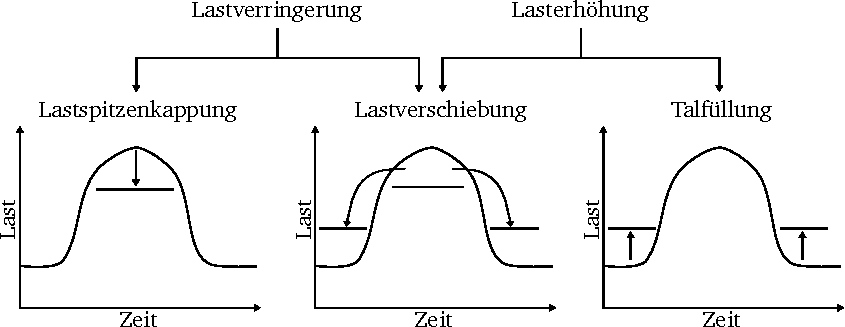
\includegraphics[width=400pt]{figures/03_Grundlagen/Lastanpassungsstrategien.pdf}
	\caption{Lastanpassungsstrategien, nach \cite{waltherMethodologyClassificationCharacterisation2022}}
	\label{fig_03Lastanpassungsstrategien}
\end{figure}

Nach der VDI-Richtlinie \cite{VDI5207Blatt2020} lassen sich sämtliche Strategien der Lastanpassung entweder reaktiv oder proaktiv realisieren. Eine Lastanpassung wird bspw. als proaktiv bezeichnet, wenn verschiedene Akteure historische Wetterdaten und Strompreisinformationen analysieren, um unterschiedliche Wetterszenarien zu prognostizieren, die zu verschieden hohen Energiepreisen führen. In diesem Kontext erfolgt die Lastanpassung im Voraus auf Basis der erwarteten Preissignale.\\

\begin{figure}[h]
	\centering
	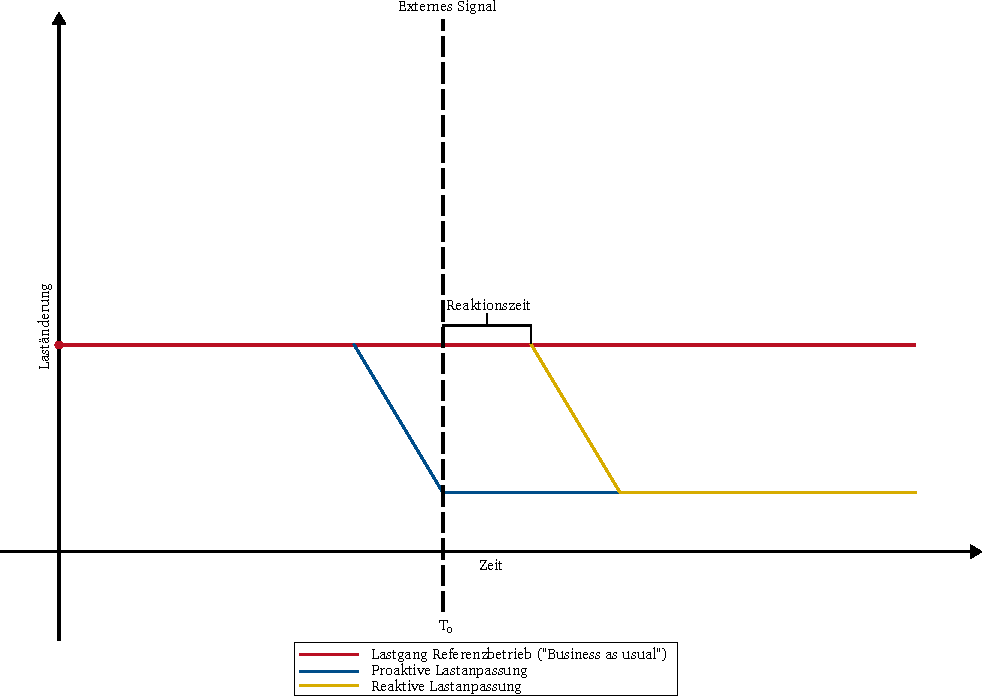
\includegraphics[width=400pt]{figures/03_Grundlagen/Pro- und Reaktive Lastanpassung.pdf}
	\caption{Pro- und Reaktive Lastanpassung, nach \cite{VDI5207Blatt2020}}
	\label{fig_03Pro- und Reaktive Lastanpassung}
\end{figure}

Ein Beispielszenario für eine reaktive Lastanpassung ist, wenn ein Industrieunternehmen von seinem Energieversorger eine Benachrichtigung erhält, dass die Strompreise aufgrund einer unvorhergesehenen Nachfragespitze in den nächsten zwei Stunden drastisch ansteigen werden. In diesem Fall muss das Unternehmen auf diese Information reagieren, indem es sofort nicht kritischen Anlagen abschaltet, um die Energiekosten zu minimieren und die Belastung des Netzes zu reduzieren. In der Abbildung \refeq{fig_03Pro- und Reaktive Lastanpassung} werden die eben definierten Szenarien verdeutlicht. Auf der x-Achse ist der zeitliche Verlauf dargestellt, während auf der y-Achse die Höhe der Last abgebildet ist.\\

Es folgt eine detailliertere Erläuterung des in Abbildung \refeq{fig_03Lastanpassungsstrategien} dargestellten Flexibilitätsziels der Lastspitzenkappung bzw. Lastspitzenglättung. Die Lastspitzenkappung (Peak Clipping) wird in der Abbildung \refeq{fig_03Lastanpassungsstrategien} als eine Maßnahme innerhalb der Strategie der Lastverringerung dargestellt. In der Literatur werden die Begriffe Lastspitzenkappung (Peak Clipping) und Lastspitzenglättung (Peak Shaving) häufig synonym verwendet \cite{fuhrlander-volkerAutomationArchitectureDemand, dahiruComprehensiveReviewDemand2023, dharaniLoadShiftingPeak2021, waltherMethodologyClassificationCharacterisation2022}. Andere Studien unterscheiden jedoch zwischen diesen beiden Konzepten: Lastspitzenkappung wird als eine spezifische Methode der Lastspitzenglättung betrachtet, die sich primär auf das unmittelbare Kappen von Spitzenlasten konzentriert. Im Gegensatz dazu umfasst Peak Shaving eine breitere Palette von Techniken zur Lastreduktion, wie die Nutzung von Energiespeichern, die Verschiebung des Energieverbrauchs oder den Einsatz von Backup-Generatoren \cite{dharaniLoadShiftingPeak2021}.\\

Die VDI-Richtlinie \cite{VDI5207Blatt2020} definiert Lastspitzenglättung als Maßnahmen zur Reduktion von Lastspitzen im Energieverbrauch eines Nutzers. Diese Strategie beinhaltet kurzfristige und schnelle Lastreduktionen, häufig durch den gezielten Abwurf nicht kritischer Lasten, um das Auftreten hoher Spitzenlasten zu verhindern. Beide Strategien zielen darauf ab, Spitzenlasten in einem Energiesystem zu reduzieren, um die Gesamtkosten zu senken und die Netzstabilität zu verbessern. Eine Reduzierung der Gesamtkosten wird durch die Vermeidung von Spitzenlasttarifen möglich, siehe Kapitel \refeq{ch_03Strommarktdesign und Wetterprognosen}.\\

Lastspitzenglättung wird in der Regel im Rahmen einer umfassenden energieflexiblen Fabrik betrachtet. Diese wird durch die oben beschriebenen Strategien wie Lastverschiebung und Lastverzicht erreicht und führt beispielsweise dazu, dass der gleichzeitige Betrieb von energieintensiven Maschinen nicht zur Überlastung eines Stromkreises führt.\\

Diese Masterthesis orientiert sich an der Definition der VDI-Richtlinie \cite{VDI5207Blatt2020} und verwendet die Begriffe Lastspitzenkappung und Lastspitzenglättung synonym.


%Variablen werden kursiv und Konstanten aufrecht geschrieben. Indizes welche zur Eindeutigen Identifizierung dienen, wie z.B. der Strom $I_\textsf{U}$ in Phase U werden auch aufrecht (und je nach Sichtweise ohne Serifen) geschrieben. Indizes welche Variabel sind, wie bei $w_{\textsf{fb,}i}$ in Gleichung (\ref{equ_03Schreibweise1}), werden kursiv geschrieben. Operatoren, wie z.B. der Differentialoperator $\text{d} r$ im Zusammenhang (\ref{equ_03Schreibweise2}), werden aufrecht geschrieben.

%Auch der Umgang mit Einheiten ist genormt. Ein häufig gemachter Fehler ist die Einheit bei der Achsenbeschriftung von Diagrammen in eckige Klammern zu setzen. Auch werden Einheiten immer aufrecht (und ohne Serifen) dargestellt. Zwischen Zahl und Einheit gehört immer ein Leerzeichen. Um im Fließtext einen Umbruch zwischen Zahl und Einheit zu verhindern kann ein geschütztes Leerzeichen verwendet werden (Beispiel: $1\,\textsf{Nm}$). Weitere Infos zu diesem Thema sind im Ordner Umgang\_mit\_Ein\_Gr\_Var\_Konst hinterlegt.
%
%\begin{equation}
%k_\textsf{w,q} = \frac{\sum\limits_{i}^{N_\textsf{fb}} w_{\textsf{fb,}i}}{r_\textsf{Ro} - r_\textsf{Sh}}
%\label{equ_03Schreibweise1}
%\end{equation}
%
%
%\begin{equation}
%\Delta \Delta F(r) = \frac{\text{d}^4 F(r)}{\text{d} r^4}  + \frac{2}{r} \frac{\text{d}^3 F(r)}{\text{d} r^3} - %\label{equ_03Schreibweise2}
%\end{equation}
%

%Weiteres Beispiel für Matrizen:
%
%%\textbf{N}_\textsf{B} \cdot n_\textsf{B} + \textbf{C}_\textsf{S} \cdot c_\textsf{S} + \textbf{C}_\textsf{R,B} \cdot c_\textsf{R} = \textbf{E}_\textsf{B} \cdot e_\textsf{B}
%\label{equ_04ModellLuft24}
%\end{equation}
%

%
%\begin{equation}
%n_\textsf{B} = \left(\begin{array}{c} B_\textsf{1a} \\ B_\textsf{2a} \\ B_\textsf{3a} \\ B_\textsf{4} \\ B_\textsf{3b} \\ B_\textsf{2b} \end{array}\right),\, c_\textsf{S} = \left(\begin{array}{c} V_\textsf{S,1a} \\ V_\textsf{S,2a} \\ V_\textsf{S,3a} \\ V_\textsf{S,4} \\ V_\textsf{S,3b} \\ V_\textsf{S,2b} \\ V_\textsf{S,1b} \end{array}\right), \, c_\textsf{R} = \left(\begin{array}{c} V_\textsf{R,1a} \\ V_\textsf{R,1b} \end{array}\right),\, e_\textsf{B} = \left(\begin{array}{c} V_\textsf{R,2a} \\ V_\textsf{R,3a} \\ V_\textsf{R,4} \\ V_\textsf{R,3b} \\ V_\textsf{R,2b} \\ B_\textsf{1b} \end{array}\right)
%\label{equ_04ModellLuft24a}
%\end{equation}
%

%
%\begin{equation}
%\label{equ_04ModellLuft28}
%\begin{aligned}
%\textbf{E}_\textsf{B} = &\left(\begin{array}{cccccc} 
%\lambda_\textsf{fb,1} + \lambda_{\delta,1} & 0 & 0 & 0 & 0 & 0 \\
%\lambda_\textsf{fb,2} + \lambda_{\delta,2} & \lambda_\textsf{fb,2} + \lambda_{\delta,2} & 0 & 0 & 0 & 0 \\
%0 & \lambda_\textsf{fb,3} + \lambda_{\delta,3} & \lambda_\textsf{fb,3} + \lambda_{\delta,3} & 0 & 0 & 0 \\
%0 & 0 & \lambda_\textsf{fb,3} + \lambda_{\delta,3} & \lambda_\textsf{fb,3} + \lambda_{\delta,3} & 0 & 0 \\
%0 & 0 & 0 & \lambda_\textsf{fb,2} + \lambda_{\delta,2} & \lambda_\textsf{fb,2} + \lambda_{\delta,2} & 0 \\
%0 & 0 & 0 & 0 & \lambda_\textsf{fb,1} + \lambda_{\delta,1} & 0 \\
%\end{array}\right) \frac{1}{2} \\
%+ &\left(\begin{array}{cccccc} 
%0 & 0 & 0 & 0 & -\lambda_\textsf{fb,1} & 0 \\
%0 & 0 & 0 & -\lambda_\textsf{fb,2} & -\lambda_\textsf{fb,2} & 0 \\
%0 & 0 & -\lambda_\textsf{fb,3} & -\lambda_\textsf{fb,3} & 0 & 0 \\
%0 & -\lambda_\textsf{fb,3} & -\lambda_\textsf{fb,3} & 0 & 0 & 0 \\
%-\lambda_\textsf{fb,2} & -\lambda_\textsf{fb,2} & 0 & 0 & 0 & 0 \\
%-\lambda_\textsf{fb,1} & 0 & 0 & 0 & 0 & 0 \\
%\end{array}\right) \frac{1}{2} \\
%+ &\left(\begin{array}{cccccc} 
%0 & 0 & 0 & 0 & 0 & 0 \\
%0 & 0 & 0 & 0 & 0 & 0 \\
%0 & 0 & 0 & 0 & 0 & 0 \\
%0 & 0 & 0 & 0 & 0 & 0 \\
%0 & 0 & 0 & 0 & 0 & 0 \\
%0 & 0 & 0 & 0 & 0 & A_\textsf{1b} \\
%\end{array}\right)
%\end{aligned}
%\end{equation}
%

%
%\begin{equation}
%\label{equ_04ModellLuft25}
%\textbf{N}_\textsf{B} = \left(\begin{array}{cccccc} 
%A_\textsf{1a} & -A_\textsf{2a} & 0 & 0 & 0 & 0 \\
%0 & A_\textsf{2a} & -A_\textsf{3a} & 0 & 0 & 0 \\
%0 & 0 & A_\textsf{3a} & -A_\textsf{4} & 0 & 0 \\
%0 & 0 & 0 & A_\textsf{4} & -A_\textsf{3b} & 0 \\
%0 & 0 & 0 & 0 & A_\textsf{3b} & -A_\textsf{2b} \\
%0 & 0 & 0 & 0 & 0 & A_\textsf{2b} \\
%\end{array}\right)
%\end{equation}
%

%
%\begin{equation}
%\label{equ_04ModellLuft26}
%\textbf{C}_\textsf{S} = \left(\begin{array}{ccccccc} 
%\lambda_{\delta,1} & \lambda_{\delta,1} & 0 & 0 & 0 & 0 & 0 \\
%0 & \lambda_{\delta,2} & \lambda_{\delta,2} & 0 & 0 & 0 & 0 \\
%0 & 0 & \lambda_{\delta,3} & \lambda_{\delta,3} & 0 & 0 & 0 \\
%0 & 0 & 0 & \lambda_{\delta,3} & \lambda_{\delta,3} & 0 & 0 \\
%0 & 0 & 0 & 0 & \lambda_{\delta,2} & \lambda_{\delta,2} & 0 \\
%0 & 0 & 0 & 0 & 0 & \lambda_{\delta,1} & \lambda_{\delta,1} \\
%\end{array}\right)\frac{1}{2}
%\end{equation}
%

%
%\begin{equation}
%\label{equ_04ModellLuft27}
%\textbf{C}_\textsf{R,B} = \left(\begin{array}{cc} 
%-\left(\lambda_\textsf{fb,1} + \lambda_{\delta,1} \right) & \lambda_\textsf{fb,1} \\
%0 & 0 \\
%0 & 0 \\
%0 & 0 \\
%0 & 0 \\
%\lambda_\textsf{fb,1} & -\left(\lambda_\textsf{fb,1} + \lambda_{\delta,1} \right) \\
%\end{array}\right)\frac{1}{2}
%\end{equation}
%

\subsection{Preisbasierte und Anreizbasierte Demand-Response-Strategien}

DR-Maßnahmen sind entweder preis- oder anreizbasiert. Ersteres trifft zu, wenn Schwankungen des Energiepreises zu einer Anpassung des Energieverbrauchs führt. Anreizbasiert sind Sie nur dann, wenn der Verbraucher einen festen Betrag für die Bereitstellung eines bestimmten Anteil der Last erhält, der für DR zur Verfügung steht \cite{qdrBenefitsDemandResponse2006, grasslEvaluatingMeasuresAdapting2014, vardakasSurveyDemandResponse2014, palenskyDemandSideManagement2011}.

Nach \cite{qdrBenefitsDemandResponse2006} werden folgende Preis-basierte Optionen und Anreiz-basierte Programme unterschieden:\\

\textbf{Preis-basierte Optionen:}
\begin{itemize}[label={--}]
	\item \textbf{Time-of-use (TOU):}\\
	 Ein Tarifmodell, das variable Einheitspreise für den Stromverbrauch in verschiedenen Zeitabschnitten innerhalb eines 24-Stunden-Tages festlegt. Diese TOU-Tarife repräsentieren die durchschnittlichen Kosten der Stromerzeugung und -lieferung während dieser spezifischen Zeitintervalle. Durch die Einführung von TOU-Tarifen können Verbraucher ihre Energiekosten optimieren, indem sie ihren Verbrauch in Zeiten mit niedrigeren Preisen verlagern, was gleichzeitig zu einer effizienteren Nutzung der Strominfrastruktur führt.\\
	 
	\item \textbf{Real-time pricing (RTP):}\\
	Ein Preismodell, bei dem die Strompreise typischerweise stündlich variieren und die Schwankungen der Großhandelspreise für Elektrizität widerspiegeln. Kunden werden gewöhnlich auf einer Day-ahead- oder Hour-ahead-Basis über die RTP-Preise informiert. Dies ermöglicht eine präzisere Anpassung des Verbrauchs an die tatsächlichen Erzeugungskosten und fördert eine effizientere Nutzung der Ressourcen.
	
	\item \textbf{Critical Peak Pricing (CPP):}\\
	CPP-Tarife kombinieren Elemente von TOU- und RTP-Tarifen. Die Basisstruktur folgt dem TOU-Modell, wobei jedoch der übliche Spitzenlastpreis unter bestimmten Auslösebedingungen, wie beispielsweise Gefährdung der Systemzuverlässigkeit oder extrem hohe Versorgungspreise, durch einen deutlich höheren CPP-Ereignispreis ersetzt wird. Diese Anpassung ermöglicht eine gezielte Reaktion auf außergewöhnliche Belastungen im Stromnetz und trägt zur Stabilisierung und Effizienzsteigerung des Systems bei.\\
\end{itemize}

\textbf{Anreiz-basierte Programme:}
\begin{itemize}[label={--}]
	\item \textbf{Direct load control:}\\
	Ein Programm, bei dem der Anbieter elektrische Geräte von Kunden, wie Klimaanlagen oder Warmwasserbereiter, kurzfristig und aus der Ferne ein- oder ausschaltet. Diese Programme richten sich vorwiegend an private Haushalte und kleine Gewerbebetriebe. Durch die Implementierung solcher Programme können Netzbetreiber Lastspitzen effizienter bewältigen und die Netzstabilität verbessern, indem sie den Stromverbrauch in Spitzenzeiten gezielt reduzieren.
	
	\item \textbf{Interruptible/curtailable (I/C) service:}\\
	Diese Tarife beinhalten Optionen zur Lastreduktion, die Kunden Preisnachlässe oder Rechnungsgutschriften bieten, wenn sie einer Reduzierung des Stromverbrauchs bei Systemausfällen zustimmen. Sollte die Lastreduktion nicht eingehalten werden, können Strafzahlungen fällig werden. Solche unterbrechbaren Programme wurden traditionell nur den größten industriellen oder gewerblichen Kunden zur Verfügung gestellt. Durch diese Programme wird die Netzstabilität in Notfällen unterstützt und die Belastung der Strominfrastruktur kann effektiver gemanagt werden.
	
	\item \textbf{Demand Bidding/Buyback-Programs:}\\
	In diesen Programmen geben Kunden Gebote zur Lastreduktion basierend auf den Stromgroßhandelspreisen oder einem entsprechenden Angebot ab. Diese Programme richten sich hauptsächlich an Großkunden, die in der Regel einen Stromverbrauch von einem Megawatt (MW) oder mehr haben. Durch diese Initiativen können Großverbraucher aktiv zur Netzstabilität beitragen und gleichzeitig von finanziellen Anreizen profitieren.
	
	\item \textbf{Emergency Demand Response Programs:}\\
	Diese Programme bieten Kunden finanzielle Anreize, um ihren Stromverbrauch in Zeiten von Reservemangel zu reduzieren. Solche Initiativen helfen, die Netzstabilität während kritischer Perioden zu sichern und verhindern potenzielle Stromausfälle.
	
	\item \textbf{Capacity Market Programs:}\\
	Diese Programme ermöglichen es Kunden, durch Lastabschaltungen als Systemkapazität zur Verfügung zu stehen, um herkömmliche Erzeugungs- oder Lieferressourcen zu ersetzen. Üblicherweise werden Kunden am Tag des Ereignisses benachrichtigt. Die Teilnehmer erhalten Vorauszahlungen für ihre Bereitschaft zur Reduktion, jedoch werden Strafen verhängt, falls sie die erforderliche Lastreduzierung nicht umsetzen. Diese Programme unterstützen die Stabilität und Effizienz des Stromnetzes durch die Optimierung der Nutzung vorhandener Ressourcen.
	
	\item \textbf{Ancillary Services Market Programs:}\\
	Kunden bieten auf den Märkten der unabhängigen Systembetreiber (ISO) oder regionalen Übertragungsorganisationen (RTO) Lastabschaltungen als Betriebsreserven an. Wenn ihre Gebote angenommen werden, erhalten sie den Marktpreis für ihre Bereitschaft zur Lastreduktion. Wird die Lastabschaltung erforderlich, ruft die ISO/RTO die Kunden zur Umsetzung auf, und sie können den Spotmarktpreis für die bereitgestellte Energie erhalten. Diese Programme helfen, die Betriebssicherheit und Flexibilität des Stromnetzes zu erhöhen.	
\end{itemize}

Die beschriebenen Demand-Response-Instrumente bieten Produktionssystemen die Möglichkeit, durch eine Anpassung ihres Energieverbrauchs an die variierenden Energiekosten signifikante Kosteneinsparungen im Vergleich zu Festpreistarifen zu realisieren. Dies wird erreicht, indem der Energieverbrauch in Zeiten hoher Energiekosten reduziert und in Zeiten niedriger Energiekosten erhöht wird. Voraussetzung dafür ist, dass die Produktionssysteme ihren Energiebedarf präzise kennen und über die Fähigkeit verfügen, diesen flexibel anzupassen. Das bedeutet, dass Produktionssysteme eine hohe Energieflexibilität aufweisen müssen.

Die Abbildung \refeq{fig_03Kategorisierung der DR-Instrumente} zeigt die verschiedenen Preis-basierten und Anreiz-basierten DR-Instrumente im Kontext ihrer zeitlichen Reaktionsfähigkeit.

\begin{figure}[h]
	\centering
	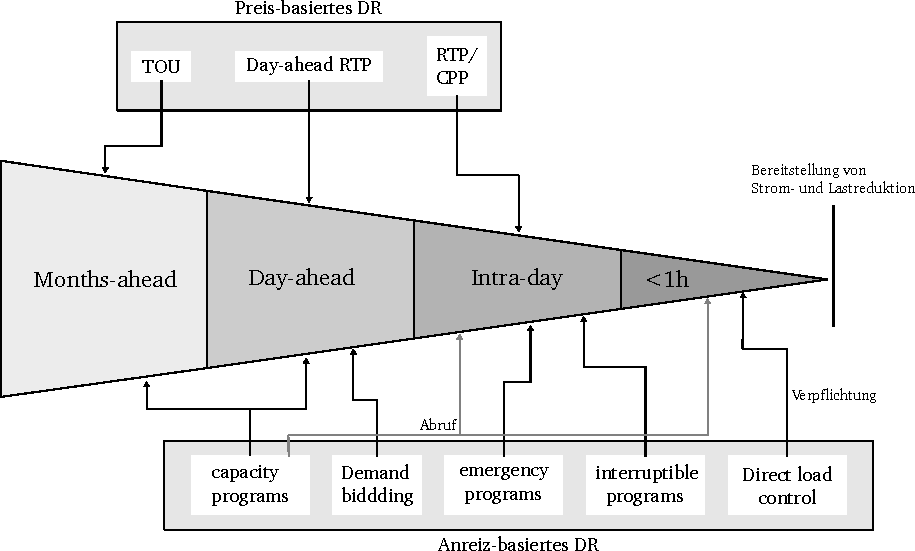
\includegraphics[width=400pt]{figures/03_Grundlagen/Kategorisierung der DR-Instrumente.pdf}
	\caption{Kategorisierung der DR-Instrumente, nach \cite{qdrBenefitsDemandResponse2006, grasslEvaluatingMeasuresAdapting2014}}
	\label{fig_03Kategorisierung der DR-Instrumente}
\end{figure}

In der Abbildung \refeq{fig_03Kategorisierung der DR-Instrumente} sind die Preis-basierten Optionen, wie TOU, Day-ahead RTP und RTP/CPP, auf der linken Seite dargestellt. Diese Instrumente ermöglichen eine Anpassung des Energieverbrauchs über längere Zeiträume, angefangen bei Monaten im Voraus bis zu weniger als einer Stunde vor dem Ereignis.\\

Die anreizbasierten Programme, einschließlich Kapazitätsprogramme, Demand Bidding, Notfallprogramme, unterbrechbare Programme und direkte Laststeuerung, sind auf der rechten Seite abgebildet. Diese Programme bieten flexiblere und schnellere Reaktionsmöglichkeiten, da sie oft eine sofortige oder kurzfristige Anpassung des Verbrauchs erfordern. Die Abbildung verdeutlicht, wie verschiedene Demand-Response-Instrumente in Abhängigkeit von der zeitlichen Dringlichkeit eingesetzt werden können, um die Netzstabilität zu gewährleisten und die Effizienz der Stromnutzung zu optimieren.\\

Die beschriebenen preis- und anreizbasierten DR-Instrumente spielen eine entscheidende Rolle im modernen Strommarktdesign. Sie bieten nicht nur flexible Lösungen zur Anpassung des Energieverbrauchs an die variierenden Marktbedingungen, sondern tragen auch wesentlich zur Stabilisierung des Stromnetzes bei.\\

Abbildung \refeq{fig_03Kategorisierung der DR-Instrumente} verdeutlicht, wie verschiedene DR-Instrumente in Abhängigkeit von der zeitlichen Dringlichkeit und der spezifischen Marktbedingungen eingesetzt werden können. Diese Instrumente sind integraler Bestandteil eines effizienten Strommarktdesigns, da sie die Nachfrage auf intelligente Weise steuern und somit die Notwendigkeit kostspieliger Spitzenlastkapazitäten reduzieren.\\

Im Kontext eines dynamischen Strommarkts sind präzise Wetterprognosen von entscheidender Bedeutung. Wetterbedingungen beeinflussen die Erzeugung erneuerbarer Energien wie Wind- und Solarenergie erheblich, was wiederum direkte Auswirkungen auf die Verfügbarkeit und die Kosten von Elektrizität hat. Durch die Integration genauer Wettervorhersagen in das Strommarktdesign können Versorgungsunternehmen und Netzbetreiber die Effizienz der Demand-Response-Instrumente weiter steigern und die Netzstabilität gewährleisten.\\

Das folgende Kapitel \refeq{ch_03Strommarktdesign und Wetterprognosen} wird sich daher mit dem Strommarktdesign und der Rolle von Wetterprognosen befassen. Dabei wird untersucht, wie diese Elemente zusammenwirken, um eine optimale Nutzung der Demand-Response-Instrumente zu ermöglichen und gleichzeitig die Herausforderungen eines zunehmend volatilen Strommarktes zu meistern.
\section{Strommarktdesign und Wetterprognosen}
\label{ch_03Strommarktdesign und Wetterprognosen}
\begin{itemize}
	\item Struktur und Funktionsweise des Strommarkts
	\item Bedeutung für die Energieflexibilisierung 
	\item Bedeutung von Wetterprognosen und deren Einfluss auf die Energieverfügbarkeit
\end{itemize}

\subsection{Struktur und Funktionsweise der Strommärkte}
In Abbildung \refeq{fig_03Vertragsbeziehungen zwischen den Akteuren am Strommarkt} sind die Vertragsbeziehungen zwischen den verschiedenen Akteuren des Strommarktes dargestellt. Diese Beziehungen bilden das Rückgrat des Strommarktdesigns und ermöglichen eine effiziente und zuverlässige Stromversorgung. Im Folgenden wird eine detaillierte Beschreibung der einzelnen Akteure des Strommarktes präsentiert, um ihre jeweiligen Rollen und Verantwortlichkeiten innerhalb des Systems zu verdeutlichen.\\
\begin{figure}[h]
	\centering
	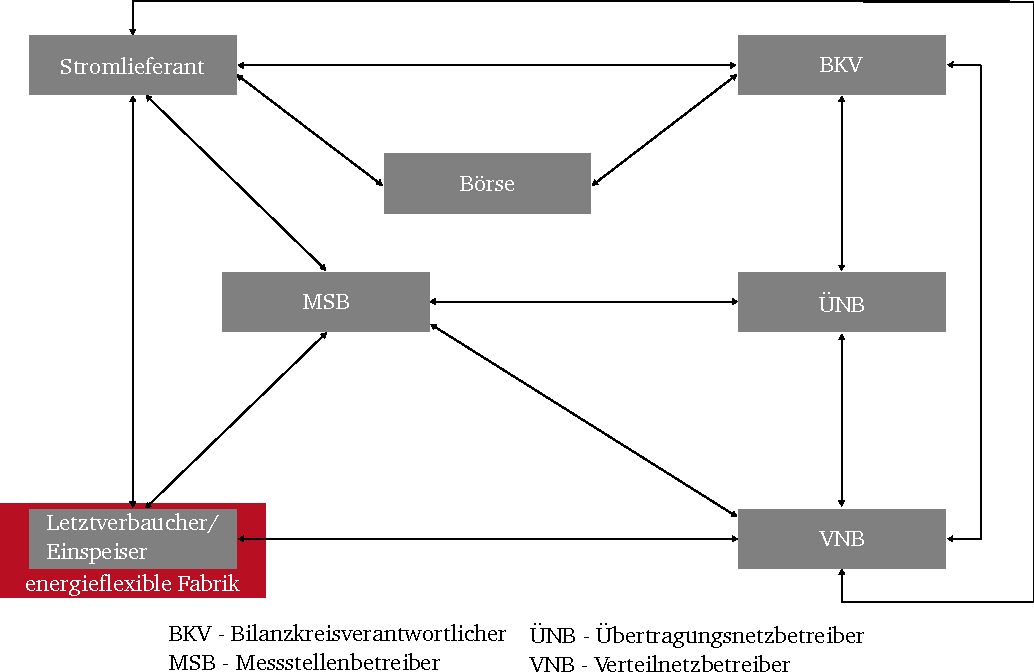
\includegraphics[width=400pt]{figures/03_Grundlagen/Vertragsbeziehungen zwischen den Akteuren am Strommarkt.pdf}
	\caption{Vertragsbeziehungen zwischen den Akteuren am Strommarkt, nach \cite{VDI5207Blatt2020}}
	\label{fig_03Vertragsbeziehungen zwischen den Akteuren am Strommarkt}
\end{figure}

Übertragungsnetzbetreiber (ÜNB) sind für den Betrieb und die Instandhaltung der Höchst- und Hochspannungsnetze verantwortlich. Diese Netze transportieren Strom über große Entfernungen und sorgen für die Einspeisung in die Verteilnetze sowie die Aufnahme von Energie aus diesen Netzen. In Deutschland gibt es vier ÜNBs: Amprion, TransnetBW, TenneT und 50Hertz. Gemäß § 12 des Energiewirtschaftsgesetzes (EnWG) sind diese Betreiber verpflichtet, die Versorgungssicherheit zu gewährleisten. Dazu erbringen sie wichtige Systemdienstleistungen wie Frequenzhaltung, Spannungshaltung, Betriebsführung und den Wiederaufbau der Versorgung nach Störungen. Die ÜNBs spielen auch eine zentrale Rolle bei der Integration erneuerbarer Energien in das Stromnetz, da sie die schwankende Einspeisung von Wind- und Solarenergie managen müssen \cite{VDI5207Blatt2020, hammonsIntegratingRenewableEnergy2008}.\\

Verteilnetzbetreiber (VNB) sind für den Betrieb und die Verwaltung der Verteilnetze verantwortlich, welche die Mittelspannungsebene (und teilweise auch die Hochspannungsebene in großen städtischen Gebieten) sowie alle darunterliegenden Spannungsebenen und Umspannstationen umfassen. Ihre gesetzliche Verpflichtung besteht darin, ein sicheres, zuverlässiges und leistungsfähiges Energieversorgungsnetz diskriminierungsfrei zu betreiben, zu warten und bei Bedarf zu optimieren, zu verstärken und auszubauen, sofern dies wirtschaftlich vertretbar ist. In Deutschland gibt es etwa 900 VNBs, die eine zentrale Rolle in der Stromverteilung spielen. Ein wichtiger Aspekt der VNBs ist ihre Beteiligung an DR-Programmen. VNBs stellen zudem Messdienste bereit, die genaue Verbrauchsdaten erfassen und an andere Marktteilnehmer wie ÜNBs und Stromlieferanten weiterleiten. Diese Daten sind essentiell für die Abrechnung und die Planung des Energiebedarfs \cite{VDI5207Blatt2020, stanelyteOverviewDemandResponseServices2022}.\\

Messstellenbetreiber (MSB) in Deutschland spielen eine zentrale Rolle im Energiemarkt, indem sie die Installation und den Betrieb von modernen Messeinrichtungen und intelligenten Messsystemen (Smart Meter) sicherstellen. Gemäß der VDI 5207 Blatt 1 \cite{VDI5207Blatt2020} kann jeder Endverbraucher seinen MSB frei wählen. Die MSBs sind für die Bereitstellung und den Betrieb dieser Messsysteme verantwortlich, die genaue Verbrauchsdaten erfassen und diese über das Smart Meter Gateway an berechtigte Marktteilnehmer weiterleiten. Moderne Messeinrichtungen und intelligente Messsysteme tragen erheblich zur Transparenz und Effizienz im Energiemarkt bei. Durch die präzise Erfassung von Echtzeitdaten ermöglichen sie eine bessere Planung und Optimierung des Energieverbrauchs, was sowohl ökonomische als auch ökologische Vorteile bietet \cite{VDI5207Blatt2020, rindSmartEnergyMeters2023}.\\

Stromlieferanten spielen eine zentrale Rolle im Strommarkt, indem sie elektrische Energie an Endverbraucher verkaufen. Sie beziehen den Strom entweder direkt von Erzeugern oder über Handelsplattformen wie die Börse und verteilen ihn an Haushalte, Unternehmen und industrielle Abnehmer. Die Preisgestaltung erfolgt in der Regel durch die Kombination von variablen Kosten pro verbrauchter Kilowattstunde und festen Grundgebühren, die unabhängig vom individuellen Verbrauch anfallen und für die Wartung des Stromnetzes sowie der Zähler zuständig sind \cite{VDI5207Blatt2020}.\\

Bilanzkreisverantwortliche (BKV) nehmen im Strommarkt eine zentrale Position ein, indem sie das Gleichgewicht zwischen Erzeugung und Verbrauch bzw. der Einspeisung und Entnahme von Strom innerhalb eines Bilanzkreises sicherstellen. Sie fungieren als wichtige Schnittstellen zwischen Verbrauchern und ÜNBs. Die Hauptaufgaben der BKVs umfassen die Erstellung von Prognosen für den Energieverbrauch und die Energieerzeugung sowie die Entwicklung von Handelsstrategien, um dieses Gleichgewicht zu gewährleisten. BKVs überwachen kontinuierlich den Zustand ihres Bilanzkreises und greifen bei Abweichungen zwischen prognostizierten und tatsächlichen Werten ein. Dazu gehören Maßnahmen wie der Handel von Ausgleichsenergie am Regelenergiemarkt, um kurzfristige Ungleichgewichte auszugleichen und die Netzstabilität zu gewährleisten \cite{VDI5207Blatt2020, wawerElektrizitaetswirtschaftPraxisorientierteEinfuehrung2022}.\\ 

Letztverbraucher, zu denen Unternehmen, energieflexible Fabriken und Haushalte zählen, wählen ihren Stromlieferanten basierend auf Kriterien wie Strommix, Preisgestaltung und vertraglichen Bedingungen. Diese Verbraucher zahlen dem gewählten Lieferanten den vereinbarten Strompreis. In einigen Fällen handeln Unternehmen direkt an der Börse oder beauftragen Dienstleister wie Direktvermarkter oder Aggregatoren, um den benötigten Strom zu beschaffen. Dadurch treten sie selbst als Lieferanten auf \cite{VDI5207Blatt2020}. Die Hauptaufgaben der Stromerzeuger und Einspeiser bestehen darin, elektrische Energie zu erzeugen und diese in die Übertragungs- oder Verteilnetze einzuspeisen, abhängig von ihrer Leistungskapazität. Anschließend verkaufen die Erzeuger den produzierten Strom an Handelsplätzen wie der Börse \cite{bardtWettbewerblicherStrommarktFuer2014}.\\

Die dargestellten Vertragsbeziehungen verdeutlichen die komplexe Interaktion zwischen den verschiedenen Akteuren des Strommarktes und unterstreichen die Notwendigkeit einer koordinierten Zusammenarbeit zur Sicherstellung einer stabilen und effizienten Stromversorgung.\\

\subsection{Bedeutung der Marktsegmente}

Abbildung \refeq{fig_03Deutscher Strommarkt} zeigt die verschiedenen Märkte, die für den Handel mit Strom und Flexibilität in Betracht kommen. Diese Märkte haben jeweils spezifische Zugangsbedingungen, einschließlich technischer Anforderungen und Handelslizenzen, die oft mit hinterlegten Bankbürgschaften verknüpft sind. Sollte ein Unternehmen diese Voraussetzungen nicht erfüllen, besteht die Möglichkeit der Teilnahme über einen Stromlieferanten oder Aggregator.

Nach der Betrachtung der einzelnen Akteure und ihrer Rollen im Strommarkt ist es nun entscheidend, die verschiedenen Marktsegmente zu erläutern, die die Grundlage für den Handel und die Preisfindung bilden. Im nächsten Abschnitt wird zunächst die Funktion und Bedeutung der Börse im Strommarkt beschrieben, bevor auf die unterschiedlichen Marktsegmente wie Spotmarkt, Terminmarkt und Regelenergiemarkt eingegangen wird.\\

\begin{figure}[h]
	\centering
	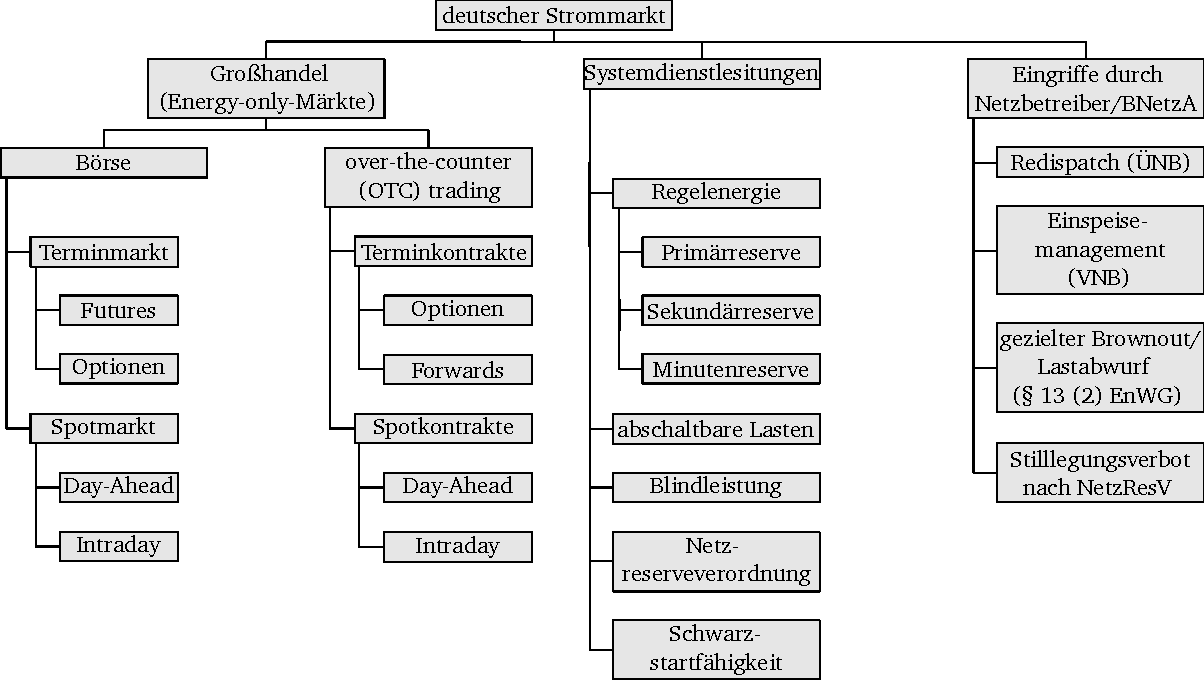
\includegraphics[width=400pt]{figures/03_Grundlagen/Deutscher Strommarkt.pdf}
	\caption{Deutscher Strommarkt, nach \cite{VDI5207Blatt2020}}
	\label{fig_03Deutscher Strommarkt}
\end{figure}
(Linien müssen überarbeitet werden, teilweise nicht genau aufeinander und dicker als die anderen)\\

Der Begriff Energy-only-Märkte bezeichnet alle Energiemärkte, auf denen tatsächliche Stromlieferungen (in Megawattstunden, MWh) kurz vor ihrer Lieferung gehandelt werden. Diese Märkte operieren auf Basis von Angebot und Nachfrage. Preissignale in diesen Märkten lenken sowohl Investitionen als auch den kurzfristig optimalen Einsatz von Ressourcen seitens Erzeugern und Verbrauchern, was aus volkswirtschaftlicher Sicht von Bedeutung ist. Zudem bieten die unterschiedlichen Marktsegmente Möglichkeiten zur Risikominderung durch Hedging, bei dem Finanzkontrakte zur Absicherung bestehender Risiken eingesetzt werden, sowie zur Arbitrage, wo Preisunterschiede zur Gewinnsteigerung genutzt werden können (betriebswirtschaftliche Perspektive). Der Handel findet sowohl an Börsen als auch bilateral über sogenannte Over-the-Counter-Geschäfte (OTC) statt \cite{VDI5207Blatt2020}.\\

Der Handel mit Strom erfolgt an spezialisierten Börsen und ist damit vergleichbar mit dem Aktienhandel. Ein prominentes Beispiel ist die European Energy Exchange (EEX), an der unter anderem auch der Strom für Deutschland gehandelt wird. Es gibt jedoch weitere Börsen, an denen Strom gehandelt wird, wie etwa die Nord Pool oder die Power Exchange Central Europe (PXE).\\

Ein wesentlicher Vorteil des Börsenhandels gegenüber dem OTC-Markt liegt in der hohen Liquidität. Börsen bieten eine standardisierte und transparente Handelsumgebung, die das Risiko für die Marktteilnehmer reduziert und eine verlässliche Preisbildung ermöglicht.\\

An den Strombörsen werden sowohl Spot- als auch Termin- bzw. Future-Kontrakte gehandelt:
Einheiten müssen hier noch als Formel formuliert werden
\begin{itemize}[label={--}]
	
\item \textbf{Spotmarkt:}\\ Der Spotmarkt umfasst Produkte im Stunden- und Viertelstundenraster. Dazu zählen der Day-Ahead-Markt, bei dem Strom für den folgenden Tag gehandelt wird, und der Intraday-Markt, der den kontinuierlichen Kauf und Verkauf von Strom für die Lieferung am selben Tag ermöglicht.\\

Im Day-Ahead-Handel, der an der EEX Spot oder im OTC-Handel stattfindet, können an jedem Tag des Jahres bis 12:00 Uhr mittags Gebote für den kommenden Tag abgegeben werden. Es werden verschiedene Produkte gehandelt, einschließlich voller Stunden und standardisierter Blockgebote, mit einer Mindesthandelseinheit von 0,1 MW und einer maximalen Blockgebotsgröße von 400 MW. Die Auktionsergebnisse, einschließlich des Markträumungspreises, werden um 12:40 Uhr veröffentlicht. Der Markträumungspreis wird durch den Schnittpunkt von Angebots- und Nachfragegeboten bestimmt, was diese Auktion zu einer Einheitspreisauktion macht.\\

Intraday-Märkte ermöglichen den kurzfristigen Stromhandel bis kurz vor der physikalischen Lieferung in viertelstündigen Intervallen. Es gibt eine Eröffnungsauktion sowie einen kontinuierlichen Handel. Die Preisspanne reicht von –9999 EUR/MWh bis +9999 EUR/MWh. Angesichts der zunehmenden Einspeisung erneuerbarer Energien sind diese Märkte besonders wichtig, um auch untertägig auf Preisschwankungen, beispielsweise durch korrigierte Wetterprognosen, reagieren zu können.\\

Diese standardisierten Produkte optimieren die Beschaffung und den Verkauf von Strom und bieten technisch-wirtschaftlich-rechtliche Sicherheiten. Sie ermöglichen es den Marktteilnehmern, Marktpreisrisiken je nach spezifischem Bedarf auszugleichen.\\

\item \textbf{Termin- bzw. Future-Kontrakte:}\\ Termin- bzw. Future-Kontrakte ermöglichen die langfristige Absicherung von Energielieferungen durch den Handel in Wochen-, Monats-, Quartals- und Jahresblöcken. Diese Kontrakte bieten den Marktteilnehmern die Möglichkeit, sich gegen zukünftige Preisschwankungen abzusichern und eine stabile Planungsgrundlage zu schaffen. Darüber hinaus erlauben sie eine Optimierung des Portfolios und die finanzielle Absicherung zukünftiger Liefergeschäfte. Der Handel kann sowohl an der Börse als auch über OTC-Geschäfte (Over-the-Counter) erfolgen. An der Börse ist der Handel bis zu sechs Jahre im Voraus möglich. Mit Futures kann man sich gegen Preisspitzen und Preistiefs absichern. Durch die Optionen können Wochen-, Monats-, Quartals- und Jahres-Futures im Peakload (8:00 - 20:00 Uhr) oder Baseload (24-Stunden-Block) gehandelt werden. Diese Kontrakte sind besonders wichtig als Mittel zur Risikoabsicherung für die fluktuierende Erzeugung erneuerbarer Energien oder für Marktpreisspitzen, die durch den wachsenden Anteil erneuerbarer Energien bedingt sind.
\end{itemize}

Der physische Stromfluss erfolgt unabhängig vom Handel über die Netzbetreiber, die je nach Spannungsebene als ÜNBs oder VNBs fungieren. Die bilanziellen Transaktionen werden durch den BKV bis zum Letztverbraucher abgewickelt.\\

Der Over-the-Counter (OTC)-Handel bezeichnet den bilateralen Handel von Strom, der neben dem Börsenhandel weiterhin eine gängige Methode im Spot-Geschäft darstellt. Im OTC-Handel werden Lieferverträge direkt mit den Abnehmern abgeschlossen, wodurch die Produkte individuell anpassbar sind, beispielsweise auf viertelstündlicher Basis. Die Verkaufserlöse fließen hierbei direkt vom Abnehmer zum Stromerzeuger. Der physische Stromfluss erfolgt auch im OTC-Handel über die Netzbetreiber, während die bilanzielle Abwicklung durch den Bilanzkreisverantwortlichen (BKV) bis zum Letztverbraucher erfolgt.\\

Systemdienstleistungen sind essenzielle Maßnahmen, die dazu dienen, die Stabilität und Sicherheit des Stromnetzes zu gewährleisten. Diese Maßnahmen sorgen dafür, dass die Netzfrequenz, die Spannung und die Leistungsbelastungen innerhalb festgelegter Grenzen bleiben oder nach Störungen wiederhergestellt werden. Üblicherweise werden diese Maßnahmen von den Netzbetreibern koordiniert und ausgeführt. Bei Störungen im Netz werden marktbezogene Interventionen wie Regelenergie und Engpassmanagement eingesetzt, ebenso wie steuerbare Lasten, die je nach Bedarf zu- oder abgeschaltet werden können. Darüber hinaus stehen Reservekapazitäten zur Verfügung, um die Netzstabilität und die Versorgungssicherheit auch in kritischen Situationen aufrechtzuerhalten.\\

\begin{itemize}[label={--}]

\item \textbf{Regelleistungsmarkt:}\\
Der Regelleistungsmarkt spielt eine entscheidende Rolle beim kurzfristigen Ausgleich von Stromangebot und -nachfrage nach Handelsschluss bis zum Zeitpunkt der physischen Lieferung. Dies dient der Aufrechterhaltung der Netzstabilität und der Sollfrequenz von 50,0 Hz. Teilnahmeberechtigt sind nur präqualifizierte Akteure, die eine vorwettbewerbliche Eignungsprüfung bestanden haben und die technischen Voraussetzungen zur Erbringung der Regelleistung erfüllen.

\begin{itemize}[label={--}]
\item \textbf{Positive Regelenergie} wird benötigt, wenn die Nachfrage das Angebot übersteigt.
\item \textbf{Negative Regelenergie} kommt zum Einsatz, wenn die Nachfrage unter dem Angebot liegt.
\end{itemize}

Die Verantwortung für den Regelleistungsmarkt liegt bei den ÜNB. Es gibt drei Typen von Regelreserve: Primärregelleistung, Sekundärregelleistung und Minutenreserveleistung. Diese unterscheiden sich hinsichtlich ihres Zeithorizonts und ihrer Anforderungen an die Anbieter.\\

\item \textbf{Verordnung zu ab- und zuschaltbaren Lasten:}\\
Die Verordnung zu abschaltbaren Lasten regelt die Steuerung von Stromverbrauchern durch den ÜNB bei Netzengpässen. Dabei können bestimmte Lasten gezielt reduziert werden. Man unterscheidet hierbei zwischen schnell und sofort abschaltbaren Lasten. Anbieter solcher Lasten müssen spezifische technische Anforderungen erfüllen und einen Rahmenvertrag mit dem ÜNB abschließen. Die Ausschreibungen für abschaltbare Lasten sind vor allem auf industrielle Verbraucher zugeschnitten, im Gegensatz zu den Anforderungen der Regelenergie. Die Verordnung zu zuschaltbaren Lasten funktioniert ähnlich wie die Bereitstellung negativer Regelenergie. Flexible Industrieprozesse können diese Art von Last anbieten. Diese Flexibilität steht dem ÜNB zur Verfügung und kann im Falle eines Netzengpasses genutzt werden, um die Netzstabilität zu sichern.\\
\end{itemize}

Die Kapazitätsreserve ist ein zentrales Instrument, das durch das Gesetz zur Weiterentwicklung des Strommarktes eingeführt wurde, um die Systemverantwortung der Übertragungsnetzbetreiber (ÜNB) zu gewährleisten. Diese Reserve dient der Bewältigung von Netzengpässen, der Stabilisierung der Netzspannung und der Wiederherstellung der Stromversorgung nach Störungen. Für die Kapazitätsreserve kommen Anlagen infrage, die zwar momentan nicht in Betrieb sind, aber aufgrund ihrer Systemrelevanz – beispielsweise ihrer Position im Netz – von den ÜNB reaktiviert werden können. Diese Anlagen werden in die Kapazitätsreserve integriert, um bei Bedarf die Stabilität und Zuverlässigkeit des Stromnetzes sicherzustellen.\\

Im Flexibilitätsmarkt nehmen Aggregatoren eine entscheidende Position ein. Sie bündeln die Flexibilität vieler kleiner Unternehmen und bieten diese gebündelt den Netzbetreibern an. Einzelne kleine Akteure sind für Netzbetreiber meist uninteressant, da größere Flexibilitätspakete bevorzugt werden. Unternehmen, die Flexibilität zur Verfügung stellen, werden dafür finanziell entschädigt. Ein Beispiel hierfür ist die Regelenergie, die von Übertragungsnetzbetreibern (ÜNB) genutzt wird, wenn der Bedarf hoch ist, etwa bei speziellen Wetterbedingungen wie Frühnebel. In solchen Situationen können gesteuerte Industrieanlagen eine wichtige Rolle spielen. Aggregatoren übernehmen auch eine Versicherungsfunktion. Sollte ein Unternehmen vorübergehend nicht in der Lage sein, Flexibilität zu bieten, können Aggregatoren die erforderliche Flexibilität durch andere Unternehmen bereitstellen. Dies ist besonders für kleine Unternehmen vorteilhaft, da sie alleine oft nicht genügend Flexibilität anbieten können. Es besteht jedoch ein Bedarf an gesetzlicher Anpassung, da der politische Fokus derzeit noch stark auf Energieerzeugung und weniger auf das Lastmanagement gerichtet ist. Der Flexibilitätsmarkt eröffnet Möglichkeiten für verschiedene Akteure, einschließlich Unternehmen, kleinerer Betriebe und Haushalte, sich aktiv an der Netzstabilisierung zu beteiligen. Ein Beispiel dafür ist die Modellstadt Augsburg, wo auch Haushalte am Flexibilitätsmarkt teilnehmen und somit zur Netzstabilität beitragen können \cite{Projektziel}.\\ (Zitat in Zotero noch ergänzen)

\subsection{Abgaben und Umlagen}
Letztverbraucher tragen neben den Vertriebskosten des Stromlieferanten, die je nach Menge und Zeitpunkt des Stromverbrauchs variieren, auch diverse administrative Preisbestandteile. Dazu zählen die Strom- und Mehrwertsteuer sowie verschiedene Umlagen, wie die des Erneuerbare-Energien-Gesetzes (EEG), des Kraft-Wärme-Kopplungsgesetzes (KWKG) und der Stromnetzentgeltverordnung (StromNEV). Weitere Kostenpunkte sind die Umlage für abschaltbare Lasten, die Konzessionsabgabe und die Netzentgelte. Diese Abgaben und Umlagen werden jährlich von der Bundesnetzagentur festgelegt.\\


In der Abbildung \refeq{ch_09Methodenkritik und Limitation der durchgeführten Untersuchung} wird die Aufteilung des Einzelhandelspreisniveaus für Haushaltskunden im Abnahmeband von 2.500 bis 5.000 kWh pro Jahr zum 1. April 2023 dargestellt. Die größten Kostenanteile entfallen auf die Energiebeschaffung mit 40,6 \% und die Nettonetzentgelte mit 19,9 \%. Weitere bedeutende Posten sind die Umsatzsteuer (16,0 \%), Vertrieb und Marge (11,6 \%) sowie die Stromsteuer (4,5 \%). Kleinere Anteile werden durch die Konzessionsabgabe (3,6 \%), das Entgelt für Messung und Messstellenbetrieb (0,8 \%) sowie verschiedene Umlagen wie die Umlage nach KWKG, nach §19 StromNEV und die Offshore-Netzumlage abgedeckt. Diese Struktur verdeutlicht, wie sich die Kosten für Strom für Endverbraucher zusammensetzen und welche Anteile durch gesetzliche Abgaben und Umlagen beeinflusst werden.
Quelle Bundesnetzagentur muss in Zotero noch ausgebessert werden!
\begin{figure}[h]
	\centering
	\includegraphics[width=400pt]{figures/03_Grundlagen/Aufteilung des Einzelhandelspreisniveaus für Haushaltskunden für das Abnahmeband ab einschließlich 2.500 bis 5.000 kWh pro Jahr zum 1. April 2023.pdf}
	\caption{Aufteilung des Einzelhandelspreisniveaus für Haushaltskunden für das Abnahmeband ab einschließlich 2.500 bis 5.000 kWh pro Jahr zum 1. April 2023 , nach \cite{BundesnetzagenturMonitoringberichte}}
	\label{fig_03Aufteilung des Einzelhandelspreisniveaus für Haushaltskunden für das Abnahmeband ab einschließlich 2.500 bis 5.000 kWh pro Jahr zum 1. April 2023}
\end{figure}
Bild muss noch ausgebssert werden - Kreis ganz rund machen

Stromintensive Unternehmen profitieren von speziellen Regelungen bei der EEG-Umlage: Ab einem bestimmten Verbrauchsniveau zahlen sie nicht mehr den vollen Umlagebetrag. Ähnlich verhält es sich bei der KWKG-Umlage, die ebenfalls von allen Stromverbrauchern landesweit getragen wird, jedoch für besonders stromintensive Betriebe begrenzt ist.

Noch was zum Merit-Order Effekt fehlt und zur EEG-Umlage 
%Es kann auf andere Kapitel, Gleichungen, Tabellen und Abbildungen verwiesen werden über Labels. Hier Beispiele: Kapitel \ref{ch_03Grundlagen1_1}, Gleichung (\ref{equ_03Grundlagen1_1_1_2}),
%Tabelle \ref{tab_03Grundlagen1_1_1},
%Abbildung \ref{fig_03Fourier1}
%
%Es ist Sinnvoll auf die Abbildungen und Tabellen immer mit Hilfe dieser Labels zu verweisen, da die Position dieser im Text von TeX so bestimmt wird, dass sich ein gleichmäßiges Schriftbild ergibt. Hierdurch kommen die Abbildungen und Tabellen nicht immer an der Stelle zum liegen an der sie im Code eingefügt sind.
%
%Die Vergebenen Labels müssen immer eindeutig sein. Die Nummerierung bei den Labels wird von TeX immer automatisch beim kompilieren aktualisiert. Ist ein Label nicht Vorhanden beispielsweise aufgrund eines Schreibfehlers, werden an der entsprechenden Stelle Fragezeichen eingefügt, wie hier \ref{Fantasielabel}. Deshalb kann es Sinnvoll sein Stellen an denen noch etwas zu bearbeiten ist mit Fragezeichen zu kennzeichnen und am Ende das Dokument über die Suchfunktion nach Fragezeichen zu durchsuchen, um nichts zu vergessen und Fehler in den Labels zu entdecken.
%
%Bei den Quellenverweisen wird in ähnlicher Form mit Labels gearbeitet. Die Daten zu den Literaturquellen sind in der bib-Datei im bibliography-Ordner hinterlegt. In dieser Datei sind für die Literatur-Einträge auch Labels hinterlegt, welche hier z.B. \cite{Binder.2017} oder optional mit Angabe der Seitenzahl \cite[S.666]{Binder.2017} oder als Aufzählung \cite{Bianchi.2009, Kerdsup.2014, Sanada.2003, Howard.2015} aufgerufen werden können. Die bib-Datei kann entweder händisch erstellt werden (nicht zu empfehlen) oder z.B. über ein Literaturverwaltungsprogramm wie Citavi. Die Labels(bibtex-keys) können in Citavi verändert werden und werden dann beim nächsten Export der bib-Datei eingetragen.


%\subsection{Grundlagen1\_1}
%\label{ch_03Grundlagen1_1}
%Beispiel für eine Aufzählung:
%
%Bei den vereinfachenden Annahmen handelt es sich um die Folgenden \cite{Binder.2017}:
%\begin{itemize}
%\item Das Eisen wird als näherungsweise unendlich magnetisch leitfähig (ideales Eisen) angenommen $\mu_{\textsf{Fe}} \to \infty$.
%\item Das Luftspaltfeld besitzt nur eine radiale Komponente, da die Luftspaltweite $\delta$ viel kleiner ist als die Polteilung $\tau_{\textsf{P}}$. 
%\item Es wird ein ebenes zweidimensionales Feld vorausgesetzt; Randeffekte an den Enden der Maschine werden vernachlässigt.
%\item Die Spulen und die Nuten, in denen diese liegen, werden als punktförmig angenommen (\textit{Dirac}'sche Durchflutungsimpulse).
%\end{itemize}
%
%Für die Erstellung von Tabellen sei auch auf hilfreiche Seiten wie https://www.tablesgenerator.com verwiesen. 
%
%\begin{table}[h]
%	\begin{center}
%		\caption[Maschinen-Kenndaten der ausgewählten Rotorblechschnittvarianten]{Maschinen-Kenndaten der ausgewählten Rotorblechschnittvarianten für den Betriebspunkt $I_\textsf{S}=1.6\,\textsf{A}$, $\beta =55°$}
%		\begin{tabular}{c|c|c|c|c|}
%		\cline{2-5}
%		                       	    & Variante 1A & Variante 1B & Variante 2A & Variante 2B \\ \hline
%		\multicolumn{1}{|c|}{$M_\textsf{e,mean}$} & $5.39\,\textsf{Nm}$ & $5.37\,\textsf{Nm}$ & $5.32\,\textsf{Nm}$ & $5.28\,\textsf{Nm}$ \\ \hline
%		\multicolumn{1}{|c|}{$\Delta M_\textsf{e,rel}$} & $8.78\,\%$ & $8.97\,\%$ & $4.52\,\%$ & $4.33\,\%$ \\ \hline
%		\multicolumn{1}{|c|}{$\cos\left(\varphi_\textsf{S} \right)$ für $R_\textsf{S}=0$} & $0.716$ & $0.720$ & $0.719$ & $0.717$ \\ \hline
%		\multicolumn{1}{|c|}{$\max\left(M_\textsf{e} \right)$} & $5.67\,\textsf{Nm}$ & $5.64\,\textsf{Nm}$ & $5.44\,\textsf{Nm}$ & $5.42\,\textsf{Nm}$ \\ \hline
%		\multicolumn{1}{|c|}{$\min\left(M_\textsf{e} \right)$} & $5.20\,\textsf{Nm}$ & $5.16\,\textsf{Nm}$ & $5.20\,\textsf{Nm}$ & $5.19\,\textsf{Nm}$ \\ \hline
%		\end{tabular}
%		\label{tab_03Grundlagen1_1_1}
%	\end{center}
%\end{table}
%
%\subsubsection{Grundlagen1\_1\_1}
%\label{ch_03Grundlagen1_1_1}
%In Abbildung \ref{fig_03Grundlagen1_1_1_1} ist ein Beispielbild zu sehen welches mit Inkscape erstellt worden ist. Die Bildunterschrift in eckigen Klammern ist die gekürzte Version für das Abbildungsverzeichnis und in geschweiften Klammern steht die ausführliche Beschreibung. Dies gilt ebenfalls für die Tabelle \ref{tab_03Grundlagen1_1_1}. 
%
%\begin{figure}[h]
%\centering
%\def\svgwidth{400pt}
%\input{figures/03_Grundlagen/Spule_2_poliger_Motor.pdf_tex}
%\caption[Zweipoliger Motor mit einer Ständerspule und homogenem Rotor]{Zweipoliger Motor mit einer Ständerspule und homogenem Rotor: \textbf{a)} Querschnitt und Feldlinien $\vec{B}$ in Folge der Nutdurchflutung $\Theta_\textsf{Q}$; \textbf{b)} Skizze des Flussdichteverlaufs $B(x)$ und Strombelags $A_\textsf{S}(x)$ über dem Luftspaltumfang $x$, nach \cite{Binder.2017}}
%\label{fig_03Grundlagen1_1_1_1}
%\end{figure}
%
%Um die Flussdichte $B_\delta$ im Luftspalt quantitativ mit dem Stromfluss $i_\textsf{C}$ in der Wicklung in Verbindung zu bringen, werden das Gesetz vom magnetischen Hüllenfluss
%%
%\begin{equation}
%\label{equ_03Grundlagen1_1_1_1}
%\oint\limits_A \vec{B} \,\text{d}\vec{A} = 0,
%\end{equation}
%%
%der Durchflutungssatz von \textit{Ampère}
%%
%\begin{equation}
%\label{equ_03Grundlagen1_1_1_2}
%\oint\limits_C \vec{H} \,\text{d}\vec{s} = \Theta
%\end{equation}
%%
%und das Materialgesetz
%%
%\begin{equation}
%\label{equ_03Grundlagen1_1_1_3}
%\vec{B} = \mu(H) \cdot \vec{H}
%\end{equation}
%%
%benötigt \cite{Binder.2017}.
%
%\subsubsection{\textit{Fourier}-Reihenentwicklung der Felderregerkurve}
%\label{ch_03Fourier}
%Die \textit{Fourier}-Reihe einer $2\pi$-periodischen Funktion $V(\gamma)$ lässt sich in der folgenden Form darstellen \cite{Binder.2017}:
%
%\begin{equation}
%\label{equ_03Fourier1}
%V(\gamma) = V_\textsf{mean} + \sum\limits_{\nu=1,2,3...}^\infty \left \lbrack \hat{V}_{\nu\textsf{,a}} \cdot \cos(\nu \gamma) + \hat{V}_{\nu\textsf{,b}} \cdot \sin(\nu \gamma) \right \rbrack
%\end{equation}
%
%Die Amplituden der Harmonischen $\hat{V}_{\nu\textsf{, a}}$ und $\hat{V}_{\nu\textsf{, b}}$ mit den Ordnungszahlen $\nu$ berechnen sich aus den Integralen (\ref{equ_03Fourier2}) und (\ref{equ_03Fourier3}) \cite{Binder.2017}.
%%
%\begin{equation}
%\hat{V}_{\nu\textsf{, a}} = \frac{1}{\pi} \int\limits_{0}^{2\pi} V(\gamma) \cdot \cos(\nu\gamma) \,\text{d}\gamma
%\label{equ_03Fourier2}
%\end{equation}
%%
%%
%\begin{equation}
%\hat{V}_{\nu\textsf{, b}} = \frac{1}{\pi} \int\limits_{0}^{2\pi} V(\gamma) \cdot \sin(\nu\gamma) \,\text{d}\gamma
%\label{equ_03Fourier3}
%\end{equation}
%%
%Die Konstante $V_\textsf{mean}$ stellt den Mittelwert der periodischen Funktion $V(\gamma)$ dar und ergibt sich aus dem Integral (\ref{equ_03Fourier4}) \cite{Binder.2017}.
%%
%\begin{equation}
%V_\textsf{mean} = \frac{1}{2\pi} \int\limits_{0}^{2\pi} V(\gamma) \,\text{d}\gamma
%\label{equ_03Fourier4}
%\end{equation}
%%
%
%\begin{figure}[h]
%\centering
%\def\svgwidth{490pt}
%\input{figures/03_Grundlagen/Fourier_1_Spule.pdf_tex}
%\caption[Felderregerkurve $V_\textsf{C}(\gamma)$ einer Spule eines Strangs einer Einschichtwicklung]{Felderregerkurve $V_\textsf{C}(\gamma)$ einer Spule eines Strangs einer Einschichtwicklung, nach \cite{Binder.2017}}
%\label{fig_03Fourier1}
%\end{figure}
%
%\subsubsection{Luftspaltleitwert}
%\label{ch_03Nutoeffnung}
%
%Die Grafik \ref{fig_03Nutoeffnung1} wurde mit Python erstellt und als svg-Datei (Vektorgrafik) abgespeichert. Anschließend wurden in Inkscape noch kleine Korrekturen der Achsen Beschriftungen vorgenommen.
%\begin{figure}[h]
%\centering
%\def\svgwidth{340pt}
%\input{figures/03_Grundlagen/dimensionslose_Leitwertfunktion.pdf_tex}
%\caption[Berechnete dimensionslose Leitwertfunktion $\tilde{\lambda}(\gamma)$ für einen vierpoligen Stator]{Berechnete dimensionslose Leitwertfunktion $\tilde{\lambda}(\gamma)$ für einen vierpoligen Stator mit $Q=36$ Nuten}
%\label{fig_03Nutoeffnung1}
%\end{figure}
\input{texts/03_Energieflexibilisierung, Strommarktdesign und wässrige Teilreinigung Grundlagen/Wässrige Teilreinigung.tex}
\input{texts/03_Energieflexibilisierung, Strommarktdesign und wässrige Teilreinigung Grundlagen/Industrielle Kommunikation über die OPC UA Schnittstelle}


